% Options for packages loaded elsewhere
\PassOptionsToPackage{unicode}{hyperref}
\PassOptionsToPackage{hyphens}{url}
%
\documentclass[
]{article}
\usepackage{amsmath,amssymb}
\usepackage{iftex}
\ifPDFTeX
  \usepackage[T1]{fontenc}
  \usepackage[utf8]{inputenc}
  \usepackage{textcomp} % provide euro and other symbols
\else % if luatex or xetex
  \usepackage{unicode-math} % this also loads fontspec
  \defaultfontfeatures{Scale=MatchLowercase}
  \defaultfontfeatures[\rmfamily]{Ligatures=TeX,Scale=1}
\fi
\usepackage{lmodern}
\ifPDFTeX\else
  % xetex/luatex font selection
\fi
% Use upquote if available, for straight quotes in verbatim environments
\IfFileExists{upquote.sty}{\usepackage{upquote}}{}
\IfFileExists{microtype.sty}{% use microtype if available
  \usepackage[]{microtype}
  \UseMicrotypeSet[protrusion]{basicmath} % disable protrusion for tt fonts
}{}
\makeatletter
\@ifundefined{KOMAClassName}{% if non-KOMA class
  \IfFileExists{parskip.sty}{%
    \usepackage{parskip}
  }{% else
    \setlength{\parindent}{0pt}
    \setlength{\parskip}{6pt plus 2pt minus 1pt}}
}{% if KOMA class
  \KOMAoptions{parskip=half}}
\makeatother
\usepackage{xcolor}
\usepackage[margin=1in]{geometry}
\usepackage{graphicx}
\makeatletter
\def\maxwidth{\ifdim\Gin@nat@width>\linewidth\linewidth\else\Gin@nat@width\fi}
\def\maxheight{\ifdim\Gin@nat@height>\textheight\textheight\else\Gin@nat@height\fi}
\makeatother
% Scale images if necessary, so that they will not overflow the page
% margins by default, and it is still possible to overwrite the defaults
% using explicit options in \includegraphics[width, height, ...]{}
\setkeys{Gin}{width=\maxwidth,height=\maxheight,keepaspectratio}
% Set default figure placement to htbp
\makeatletter
\def\fps@figure{htbp}
\makeatother
\setlength{\emergencystretch}{3em} % prevent overfull lines
\providecommand{\tightlist}{%
  \setlength{\itemsep}{0pt}\setlength{\parskip}{0pt}}
\setcounter{secnumdepth}{-\maxdimen} % remove section numbering
\usepackage{booktabs}
\ifLuaTeX
  \usepackage{selnolig}  % disable illegal ligatures
\fi
\usepackage{bookmark}
\IfFileExists{xurl.sty}{\usepackage{xurl}}{} % add URL line breaks if available
\urlstyle{same}
\hypersetup{
  pdftitle={CinC 2025},
  hidelinks,
  pdfcreator={LaTeX via pandoc}}

\title{CinC 2025}
\author{}
\date{\vspace{-2.5em}}

\begin{document}
\maketitle

\begin{verbatim}
## -- Attaching core tidyverse packages ------------------------ tidyverse 2.0.0 --
## v dplyr     1.1.4     v readr     2.1.5
## v forcats   1.0.0     v stringr   1.5.1
## v ggplot2   3.5.1     v tibble    3.2.1
## v lubridate 1.9.3     v tidyr     1.3.1
## v purrr     1.0.2     
## -- Conflicts ------------------------------------------ tidyverse_conflicts() --
## x dplyr::filter() masks stats::filter()
## x dplyr::lag()    masks stats::lag()
## i Use the conflicted package (<http://conflicted.r-lib.org/>) to force all conflicts to become errors
## 
## Attaching package: 'MASS'
## 
## 
## The following object is masked from 'package:dplyr':
## 
##     select
## 
## 
## Loading required package: lattice
## 
## 
## Attaching package: 'caret'
## 
## 
## The following object is masked from 'package:purrr':
## 
##     lift
\end{verbatim}

\section{Methods}\label{methods}

\subsection{Dataset}\label{dataset}

\begin{verbatim}
## `summarise()` has grouped output by 'data'. You can override using the
## `.groups` argument.
\end{verbatim}

\begin{verbatim}
## # A tibble: 4 x 3
## # Groups:   data [3]
##   data    error_type n_samples
##   <chr>   <chr>          <int>
## 1 healthy train            422
## 2 healthy valid             53
## 3 iMI     valid            128
## 4 pMI     valid            176
\end{verbatim}

\begin{verbatim}
## Rows: 8 Columns: 6
## -- Column specification --------------------------------------------------------
## Delimiter: ","
## chr (4): temp_model, geom_model, results_dir, experiment_description
## dbl (2): n_temp_feats, n_geom_feats
## 
## i Use `spec()` to retrieve the full column specification for this data.
## i Specify the column types or set `show_col_types = FALSE` to quiet this message.
## New names:
## Rows: 36000 Columns: 7
## -- Column specification --------------------------------------------------------
## Delimiter: ","
## chr (1): model
## dbl (6): ...1, sd, temp_dim, frame, geom_dim, value
## 
## i Use `spec()` to retrieve the full column specification for this data.
## i Specify the column types or set `show_col_types = FALSE` to quiet this message.
## New names:
## Rows: 18000 Columns: 7
## -- Column specification --------------------------------------------------------
## Delimiter: ","
## chr (1): model
## dbl (6): ...1, sd, temp_dim, frame, geom_dim, value
## 
## i Use `spec()` to retrieve the full column specification for this data.
## i Specify the column types or set `show_col_types = FALSE` to quiet this message.
## Rows: 3150 Columns: 6
## -- Column specification --------------------------------------------------------
## Delimiter: ","
## chr (1): model
## dbl (5): sd, temp_dim, frame, geom_dim, value
## 
## i Use `spec()` to retrieve the full column specification for this data.
## i Specify the column types or set `show_col_types = FALSE` to quiet this message.
## Rows: 3550 Columns: 6
## -- Column specification --------------------------------------------------------
## Delimiter: ","
## chr (1): model
## dbl (5): sd, temp_dim, frame, geom_dim, value
## 
## i Use `spec()` to retrieve the full column specification for this data.
## i Specify the column types or set `show_col_types = FALSE` to quiet this message.
\end{verbatim}

\section{Results}\label{results}

We fit the model described in Section \[INSERT REF\] on a training set
of healthy individuals, and test the model on a healthy, incident MI and
prevalent MI cohort (healthy/iMI/pMI test.)

\subsection{Reconstruction}\label{reconstruction}

Table {[}INSERT REFERENCE{]} shows the mean and standard deviation of
the average Chamfer distance over all frames for each subject. We see
that although there is a decrease in the reconstruction quality for the
iMI and pMI groups, it is not significant, and still below the voxel
dimensions of the original images.

\begin{verbatim}
## `summarise()` has grouped output by 'error_type', 'data', 'sample'. You can
## override using the `.groups` argument.
## `summarise()` has grouped output by 'error_type', 'data'. You can override
## using the `.groups` argument.
## `summarise()` has grouped output by 'data'. You can override using the
## `.groups` argument.
\end{verbatim}

\begin{tabular}{lll}
\toprule
Population & Train & Test\\
\midrule
Healthy & 0.893 (X0.182) & 0.879 (X0.138)\\
iMI & NA & 0.961 (X0.166)\\
pMI & NA & 0.996 (X0.183)\\
\bottomrule
\end{tabular}

\subsection{MI Detection}\label{mi-detection}

We fit a logistic regression to distinguish iMI and pMI from healthy
cases from the reduced dimension temporal representations of the
anatomies. We compare this to the baseline of a logistic regression
using only features from the ED and ES phases.

\begin{verbatim}
## ***MLeval: Machine Learning Model Evaluation***
\end{verbatim}

\begin{verbatim}
## Input: caret train function object
\end{verbatim}

\begin{verbatim}
## Not averaging probs.
\end{verbatim}

\begin{verbatim}
## Group 1 type: cv
\end{verbatim}

\begin{verbatim}
## Observations: 603
\end{verbatim}

\begin{verbatim}
## Number of groups: 1
\end{verbatim}

\begin{verbatim}
## Observations per group: 603
\end{verbatim}

\begin{verbatim}
## Positive: iMI
\end{verbatim}

\begin{verbatim}
## Negative: healthy
\end{verbatim}

\begin{verbatim}
## Group: Group 1
\end{verbatim}

\begin{verbatim}
## Positive: 128
\end{verbatim}

\begin{verbatim}
## Negative: 475
\end{verbatim}

\begin{verbatim}
## ***Performance Metrics***
\end{verbatim}

\begin{verbatim}
## Group 1 Optimal Informedness = 0.254901315789474
\end{verbatim}

\begin{verbatim}
## Group 1 AUC-ROC = 0.64
\end{verbatim}

\begin{verbatim}
## ***MLeval: Machine Learning Model Evaluation***
\end{verbatim}

\begin{verbatim}
## Input: caret train function object
\end{verbatim}

\begin{verbatim}
## Not averaging probs.
\end{verbatim}

\begin{verbatim}
## Group 1 type: cv
\end{verbatim}

\begin{verbatim}
## Observations: 603
\end{verbatim}

\begin{verbatim}
## Number of groups: 1
\end{verbatim}

\begin{verbatim}
## Observations per group: 603
\end{verbatim}

\begin{verbatim}
## Positive: iMI
\end{verbatim}

\begin{verbatim}
## Negative: healthy
\end{verbatim}

\begin{verbatim}
## Group: Group 1
\end{verbatim}

\begin{verbatim}
## Positive: 128
\end{verbatim}

\begin{verbatim}
## Negative: 475
\end{verbatim}

\begin{verbatim}
## ***Performance Metrics***
\end{verbatim}

\begin{verbatim}
## Group 1 Optimal Informedness = 0.315575657894737
\end{verbatim}

\begin{verbatim}
## Group 1 AUC-ROC = 0.68
\end{verbatim}

\begin{verbatim}
## ***MLeval: Machine Learning Model Evaluation***
\end{verbatim}

\begin{verbatim}
## Input: caret train function object
\end{verbatim}

\begin{verbatim}
## Not averaging probs.
\end{verbatim}

\begin{verbatim}
## Group 1 type: cv
\end{verbatim}

\begin{verbatim}
## Observations: 651
\end{verbatim}

\begin{verbatim}
## Number of groups: 1
\end{verbatim}

\begin{verbatim}
## Observations per group: 651
\end{verbatim}

\begin{verbatim}
## Positive: pMI
\end{verbatim}

\begin{verbatim}
## Negative: healthy
\end{verbatim}

\begin{verbatim}
## Group: Group 1
\end{verbatim}

\begin{verbatim}
## Positive: 176
\end{verbatim}

\begin{verbatim}
## Negative: 475
\end{verbatim}

\begin{verbatim}
## ***Performance Metrics***
\end{verbatim}

\begin{verbatim}
## Group 1 Optimal Informedness = 0.474641148325359
\end{verbatim}

\begin{verbatim}
## Group 1 AUC-ROC = 0.79
\end{verbatim}

\begin{verbatim}
## ***MLeval: Machine Learning Model Evaluation***
\end{verbatim}

\begin{verbatim}
## Input: caret train function object
\end{verbatim}

\begin{verbatim}
## Not averaging probs.
\end{verbatim}

\begin{verbatim}
## Group 1 type: cv
\end{verbatim}

\begin{verbatim}
## Observations: 651
\end{verbatim}

\begin{verbatim}
## Number of groups: 1
\end{verbatim}

\begin{verbatim}
## Observations per group: 651
\end{verbatim}

\begin{verbatim}
## Positive: pMI
\end{verbatim}

\begin{verbatim}
## Negative: healthy
\end{verbatim}

\begin{verbatim}
## Group: Group 1
\end{verbatim}

\begin{verbatim}
## Positive: 176
\end{verbatim}

\begin{verbatim}
## Negative: 475
\end{verbatim}

\begin{verbatim}
## ***Performance Metrics***
\end{verbatim}

\begin{verbatim}
## Group 1 Optimal Informedness = 0.472715311004785
\end{verbatim}

\begin{verbatim}
## Group 1 AUC-ROC = 0.8
\end{verbatim}

\begin{verbatim}
## ***MLeval: Machine Learning Model Evaluation***
\end{verbatim}

\begin{verbatim}
## Input: caret train function object
\end{verbatim}

\begin{verbatim}
## Not averaging probs.
\end{verbatim}

\begin{verbatim}
## Group 1 type: cv
\end{verbatim}

\begin{verbatim}
## Observations: 603
\end{verbatim}

\begin{verbatim}
## Number of groups: 1
\end{verbatim}

\begin{verbatim}
## Observations per group: 603
\end{verbatim}

\begin{verbatim}
## Positive: iMI
\end{verbatim}

\begin{verbatim}
## Negative: healthy
\end{verbatim}

\begin{verbatim}
## Group: Group 1
\end{verbatim}

\begin{verbatim}
## Positive: 128
\end{verbatim}

\begin{verbatim}
## Negative: 475
\end{verbatim}

\begin{verbatim}
## ***Performance Metrics***
\end{verbatim}

\begin{verbatim}
## Group 1 Optimal Informedness = 0.3109375
\end{verbatim}

\begin{verbatim}
## Group 1 AUC-ROC = 0.7
\end{verbatim}

\begin{verbatim}
## ***MLeval: Machine Learning Model Evaluation***
\end{verbatim}

\begin{verbatim}
## Input: caret train function object
\end{verbatim}

\begin{verbatim}
## Not averaging probs.
\end{verbatim}

\begin{verbatim}
## Group 1 type: cv
\end{verbatim}

\begin{verbatim}
## Observations: 603
\end{verbatim}

\begin{verbatim}
## Number of groups: 1
\end{verbatim}

\begin{verbatim}
## Observations per group: 603
\end{verbatim}

\begin{verbatim}
## Positive: iMI
\end{verbatim}

\begin{verbatim}
## Negative: healthy
\end{verbatim}

\begin{verbatim}
## Group: Group 1
\end{verbatim}

\begin{verbatim}
## Positive: 128
\end{verbatim}

\begin{verbatim}
## Negative: 475
\end{verbatim}

\begin{verbatim}
## ***Performance Metrics***
\end{verbatim}

\begin{verbatim}
## Group 1 Optimal Informedness = 0.407779605263158
\end{verbatim}

\begin{verbatim}
## Group 1 AUC-ROC = 0.77
\end{verbatim}

\begin{verbatim}
## ***MLeval: Machine Learning Model Evaluation***
\end{verbatim}

\begin{verbatim}
## Input: caret train function object
\end{verbatim}

\begin{verbatim}
## Not averaging probs.
\end{verbatim}

\begin{verbatim}
## Group 1 type: cv
\end{verbatim}

\begin{verbatim}
## Observations: 651
\end{verbatim}

\begin{verbatim}
## Number of groups: 1
\end{verbatim}

\begin{verbatim}
## Observations per group: 651
\end{verbatim}

\begin{verbatim}
## Positive: pMI
\end{verbatim}

\begin{verbatim}
## Negative: healthy
\end{verbatim}

\begin{verbatim}
## Group: Group 1
\end{verbatim}

\begin{verbatim}
## Positive: 176
\end{verbatim}

\begin{verbatim}
## Negative: 475
\end{verbatim}

\begin{verbatim}
## ***Performance Metrics***
\end{verbatim}

\begin{verbatim}
## Group 1 Optimal Informedness = 0.43994019138756
\end{verbatim}

\begin{verbatim}
## Group 1 AUC-ROC = 0.77
\end{verbatim}

\begin{verbatim}
## ***MLeval: Machine Learning Model Evaluation***
\end{verbatim}

\begin{verbatim}
## Input: caret train function object
\end{verbatim}

\begin{verbatim}
## Not averaging probs.
\end{verbatim}

\begin{verbatim}
## Group 1 type: cv
\end{verbatim}

\begin{verbatim}
## Observations: 651
\end{verbatim}

\begin{verbatim}
## Number of groups: 1
\end{verbatim}

\begin{verbatim}
## Observations per group: 651
\end{verbatim}

\begin{verbatim}
## Positive: pMI
\end{verbatim}

\begin{verbatim}
## Negative: healthy
\end{verbatim}

\begin{verbatim}
## Group: Group 1
\end{verbatim}

\begin{verbatim}
## Positive: 176
\end{verbatim}

\begin{verbatim}
## Negative: 475
\end{verbatim}

\begin{verbatim}
## ***Performance Metrics***
\end{verbatim}

\begin{verbatim}
## Group 1 Optimal Informedness = 0.548504784688995
\end{verbatim}

\begin{verbatim}
## Group 1 AUC-ROC = 0.83
\end{verbatim}

\begin{tabular}{llrrrrr}
\toprule
data & feats & Accuracy & AUC-ROC & F1 & PREC & SENS\\
\midrule
iMI & ED + ES & 0.783 & 0.68 & 0.144 & 0.440 & 0.086\\
pMI & ED + ES & 0.782 & 0.80 & 0.517 & 0.644 & 0.432\\
iMI & Full Cycle & 0.821 & 0.77 & 0.449 & 0.647 & 0.344\\
pMI & Full Cycle & 0.794 & 0.83 & 0.562 & 0.662 & 0.489\\
\bottomrule
\end{tabular}

\subsection{Geometric Features}\label{geometric-features}

\subsection{Temporal Features}\label{temporal-features}

In this section, features that were identified as for predictive
accuracy by the logistic regression.

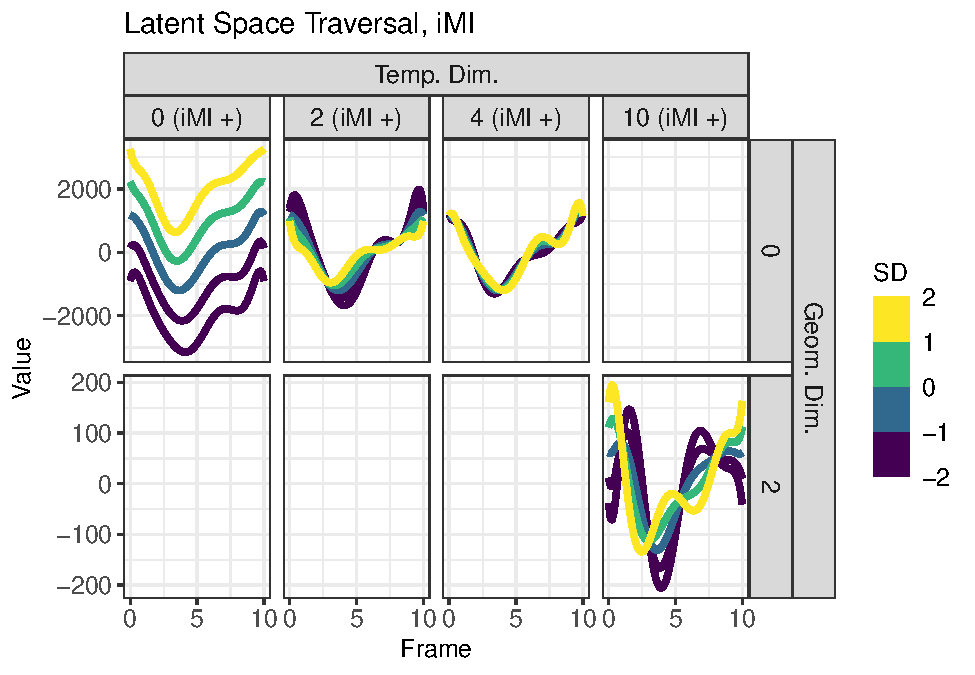
\includegraphics[width=0.5\linewidth]{cinc_2025_files/figure-latex/latent-traversal-iMI-smoothing-1}

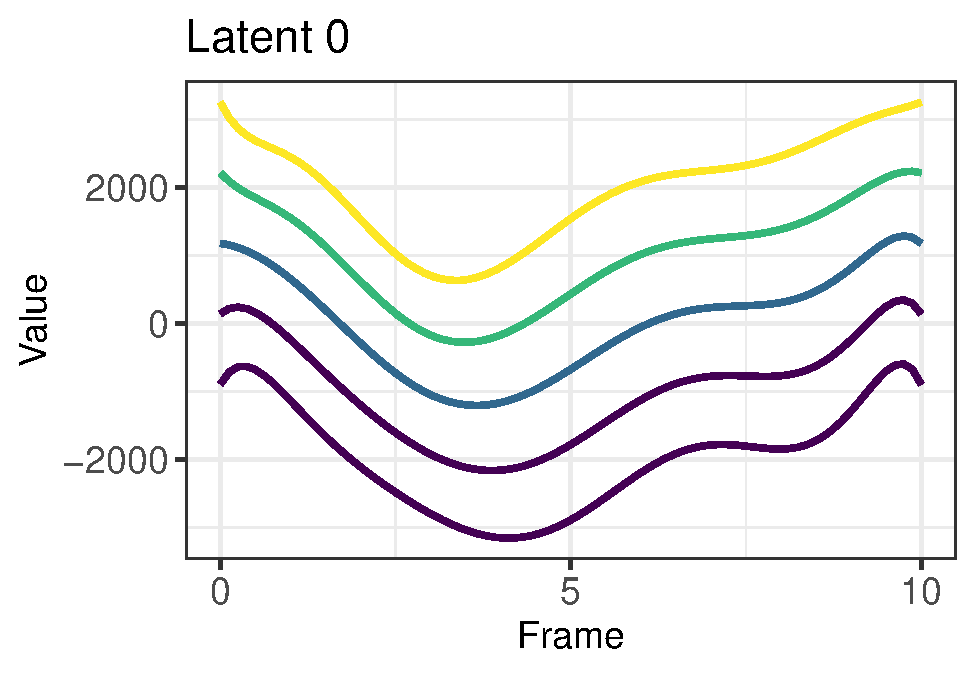
\includegraphics[width=0.5\linewidth]{cinc_2025_files/figure-latex/latent-traversal-iMI-smoothing-1-1}

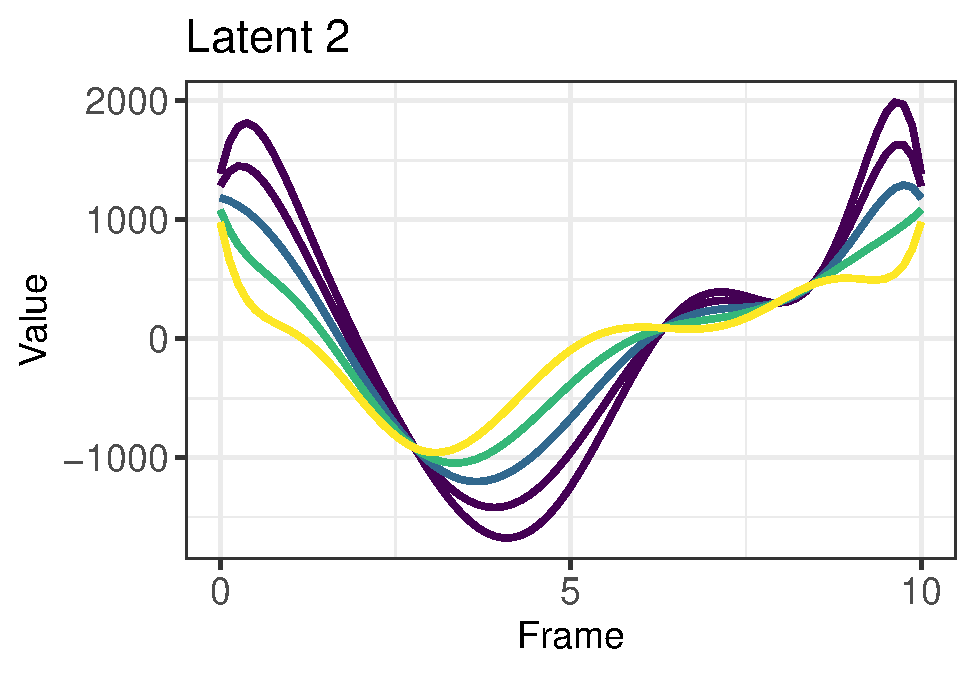
\includegraphics[width=0.5\linewidth]{cinc_2025_files/figure-latex/latent-traversal-iMI-smoothing-2-1}

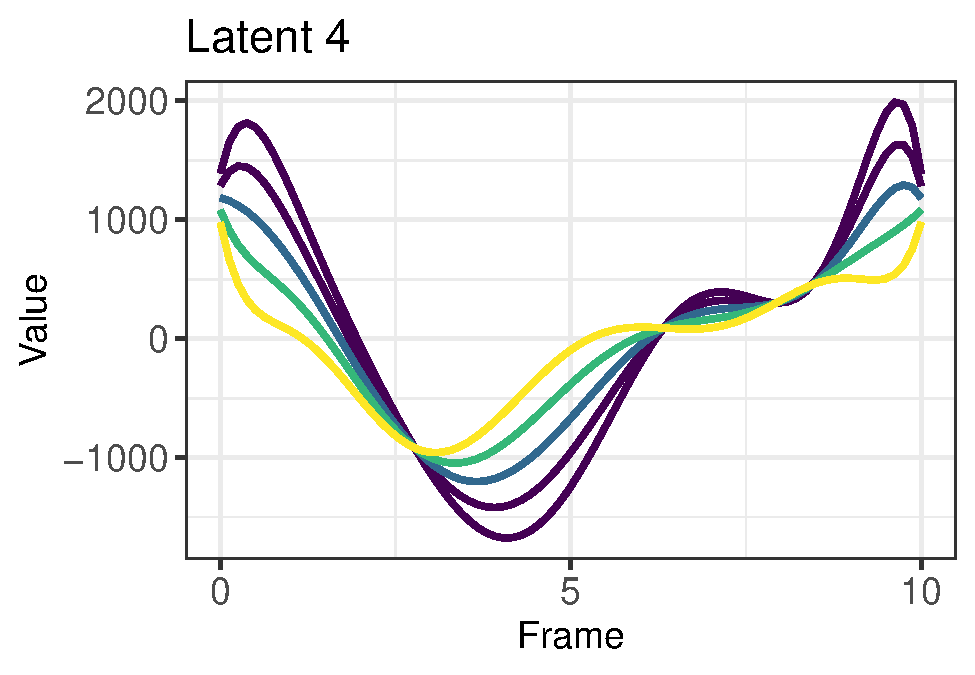
\includegraphics[width=0.5\linewidth]{cinc_2025_files/figure-latex/latent-traversal-iMI-smoothing-4-1}

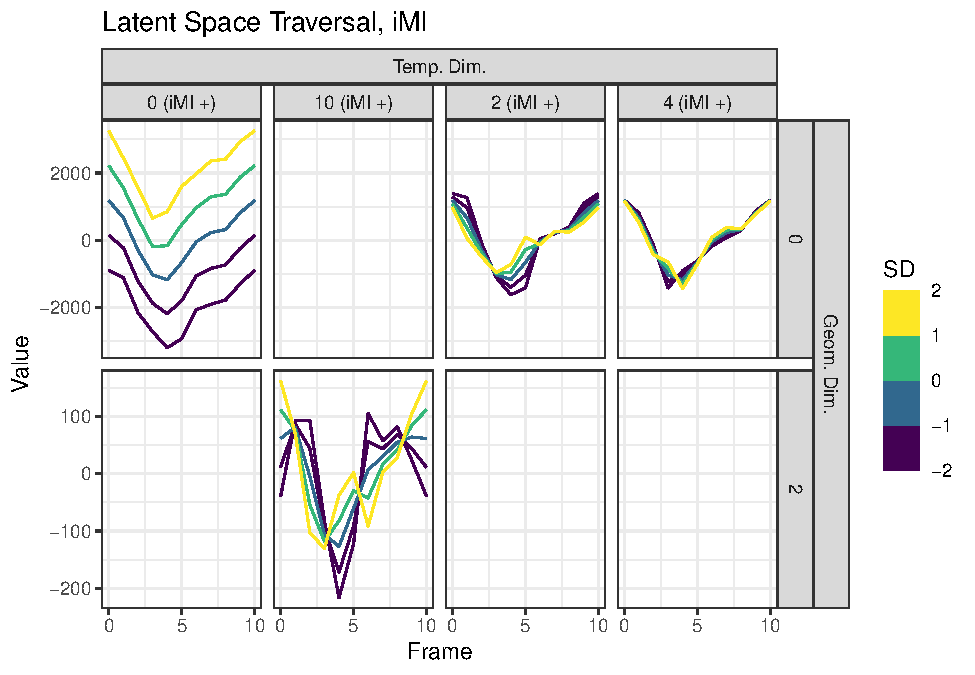
\includegraphics{cinc_2025_files/figure-latex/latent-traversal-iMI-1.pdf}

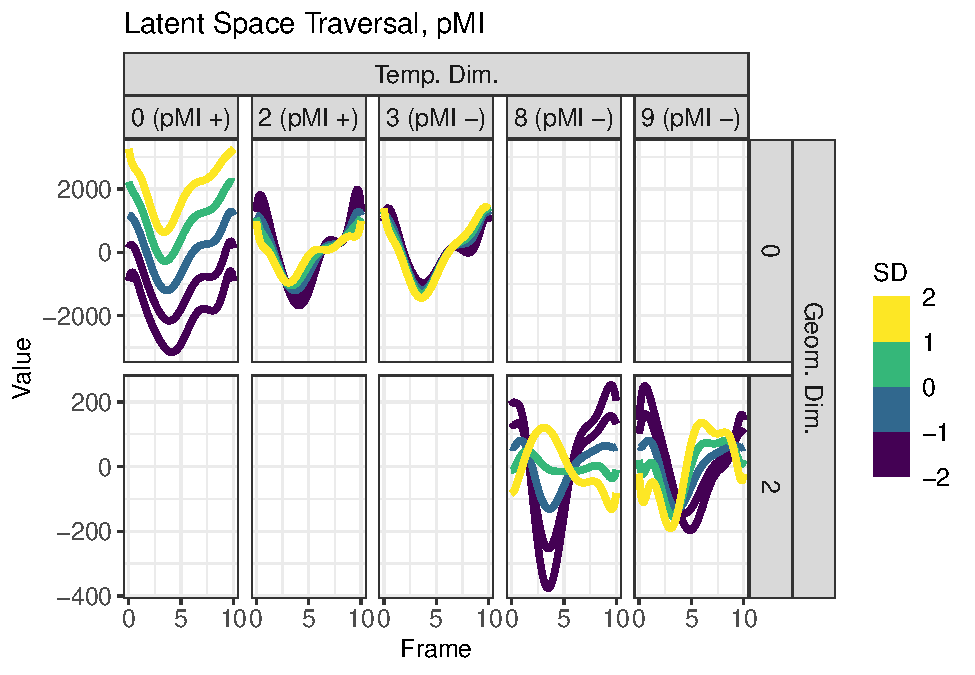
\includegraphics{cinc_2025_files/figure-latex/latent-traversal-pMI-smoothing-1.pdf}

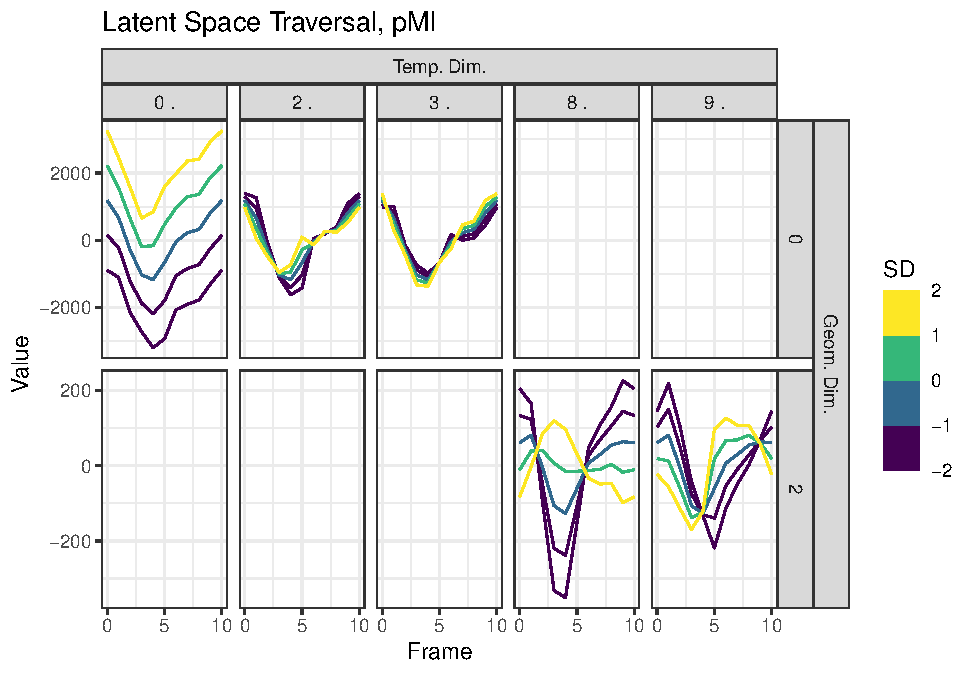
\includegraphics{cinc_2025_files/figure-latex/latent-traversal-pMI-1.pdf}
Probably want to put a 3D example just to drive the point home here. \#
Discussion

\end{document}
